\documentclass[12pt]{article}
\usepackage[utf8]{inputenc}
\usepackage[spanish]{babel}
\usepackage{amsmath}
\usepackage{booktabs}
\usepackage{geometry}
\geometry{margin=2.5cm}
\usepackage{graphicx}
\usepackage{graphicx}


\title{
Optimización del Tiempo de Atención al Cliente en un Negocio de Fotocopias Tipo Offset utilizando Programación Lineal\\[0.5em]
\large Optimization of Customer Service Time in an Offset Photocopy Business using Linear Programming
}

\author{
Mario Wilfredo Ramirez Puma \\
Angello Marcelo Zamora Valencia \\
Cliver Daniel Mamani Huatta \\
Kenny Leonel Ccora Quispe \\[0.8em]
UNIVERSIDAD NACIONAL DEL ALTIPLANO - PUNO \\
Facultad de Ingeniería Estadística e Informática
}

\date{Puno, 11 de mayo de 2025}

\begin{document}

\maketitle

\section*{Resumen}
Este trabajo presenta el desarrollo de un modelo de programación lineal para optimizar el proceso de atención al cliente en un negocio de fotocopias tipo offset ubicado en la ciudad de Puno, Perú. La atención se ve afectada por múltiples factores como el tipo de servicio solicitado, la experiencia del cliente, la disponibilidad del personal y la infraestructura. El objetivo es minimizar el tiempo total de atención diaria, mejorando así la eficiencia operativa y la satisfacción del cliente.

\section*{Abstract}
This paper presents the development of a linear programming model to optimize the customer service process in an offset photocopy business located in the city of Puno, Peru. Customer service is influenced by multiple factors such as the type of service requested, the customer's experience, staff availability, and infrastructure. The objective is to minimize the total daily service time, thereby improving operational efficiency and customer satisfaction.


\newpage
\section{Introducción}

En la actualidad, la eficiencia en la atención al cliente se ha convertido en un factor determinante para la competitividad de los negocios dedicados a la prestación de servicios. Los consumidores valoran cada vez más la rapidez y calidad del servicio recibido, y una atención ágil puede marcar la diferencia entre la preferencia o el abandono de un negocio.

En la ciudad de Puno, los establecimientos dedicados a las fotocopias tipo offset, especialmente aquellos ubicados en zonas cercanas a instituciones educativas como la Universidad Nacional del Altiplano, experimentan una alta afluencia de clientes, particularmente durante los horarios pico. Esta demanda intensa provoca frecuentemente tiempos de espera prolongados, lo cual genera insatisfacción entre los usuarios y sobrecarga a los trabajadores.

A pesar de contar con personal capacitado y maquinaria adecuada, la organización de los servicios suele realizarse de manera empírica, sin un enfoque formal de optimización. Esta falta de planificación técnica da lugar a cuellos de botella en la atención y una utilización ineficiente de los recursos disponibles.

Frente a este contexto, el presente estudio propone el uso de técnicas de programación lineal como herramienta para modelar y mejorar el proceso de atención al cliente. Mediante la formulación de un modelo matemático que considere los diferentes tipos de pedidos y los recursos disponibles, se busca minimizar el tiempo total de atención diaria. Este enfoque no solo permitirá incrementar la eficiencia operativa del negocio, sino que también contribuirá a una mejor experiencia del cliente y a una mayor competitividad en el mercado local.


\section{Materiales y Métodos}
La presente investigación tiene un enfoque cuantitativo y descriptivo, orientado al desarrollo de un modelo de programación lineal para optimizar el tiempo de atención al cliente en un negocio de fotocopias tipo offset en la ciudad de Puno.

\subsection{Contexto del Problema}

La observación directa se realizó durante 1 día hábil, abarcando un perido de 2 horas en distintos negocios de fotocopias tipo offset ubicado en las inmediaciones de la Universidad Nacional del Altiplano en la ciudad de Puno, Gracias a esta observación obtuvimos los promedios de tiempo y de tipos de clientes.
Se identificaron tres tipos de clientes:

\begin{itemize}
  \item \textbf{Clientes con pedidos simples:} Copias e impresiones sin edición.
  \item \textbf{Clientes con pedidos intermedios:} Edición básica, escaneos.
  \item \textbf{Clientes con pedidos complejos:} Encuadernados, formatos especiales.
\end{itemize}

Cada tipo de cliente requiere un tiempo promedio diferente de atención y el uso de recursos específicos.

\subsection{Variables del Modelo}

Definimos las siguientes variables de decisión:

\begin{itemize}
  \item \( x_1 \): Número de clientes con pedidos simples.
  \item \( x_2 \): Número de clientes con pedidos intermedios.
  \item \( x_3 \): Número de clientes con pedidos complejos.
\end{itemize}

Los tiempos promedio de atención para cada tipo de cliente son los siguientes:

\begin{itemize}
  \item \( t_1 = 4 \, \text{min} \) para clientes con pedidos simples.
  \item \( t_2 = 8 \, \text{min} \) para clientes con pedidos intermedios.
  \item \( t_3 = 15 \, \text{min} \) para clientes con pedidos complejos.
\end{itemize}

\subsection{Función Objetivo}

El objetivo es minimizar el tiempo total de atención diaria, expresado mediante la siguiente función lineal:

\[
\min Z = 4x_1 + 8x_2 + 15x_3
\]

\subsection{Restricciones}

Se consideran las siguientes restricciones para el modelo:

\begin{itemize}
  \item \textbf{Capacidad de atención de los empleados:} El negocio cuenta con 2 empleados que laboran 8 horas diarias (480 minutos). La capacidad total de atención no debe exceder esta cantidad.
  \[
  4x_1 + 8x_2 + 15x_3 \leq 960
  \]
  \item \textbf{Demanda mínima diaria estimada:} Se estima que deben atenderse al menos 60 clientes diariamente.
  \[
  x_1 + x_2 + x_3 \geq 60
  \]
  \item \textbf{Proporción mínima de clientes simples:} Al menos el 30\% de los clientes deben ser atendidos con pedidos simples.
  \[
  0.7x_1 - 0.3x_2 - 0.3x_3 \geq 0
  \]
  \item \textbf{Proporción máxima de clientes complejos:} No más del 40\% de los clientes pueden tener pedidos complejos.
  \[
  -0.4x_1 - 0.4x_2 + 0.6x_3 \leq 0
  \]
\end{itemize}

\subsection{Método de Solución}

El modelo de programación lineal entero fue resuelto utilizando Python y la librería \texttt{PuLP}, aplicando el método \textit{Branch and Bound} con el solucionador CBC, que es el predeterminado en esta librería.

---

Este enfoque integra ambos textos y presenta la información de manera coherente. Puedes copiar y pegar este contenido en tu documento LaTeX para que quede estructurado de forma clara y profesional.


\section{Resultados y Discusion}
El modelo propuesto sugiere una solución óptima con los siguientes valores:
\[
x_1 = 56, \quad x_2 = 30, \quad x_3 = 27
\]
\[
Z = 4(56) + 8(30) + 15(27) = 224 + 240 + 405 = 869 \text{ minutos}
\]

\subsection*{Cuadro 1: Comparación Antes vs. Después de la Optimización}

\begin{center}
\begin{tabular}{lcc}
\toprule
\textbf{Indicador} & \textbf{Antes} & \textbf{Después} \\
\midrule
Tiempo total de atención (min) & 960 & 869 \\
Clientes atendidos & 60 & 113 \\
Promedio por cliente (min) & 16.0 & 7.69 \\
\bottomrule
\end{tabular}
\end{center}
Los resultados obtenidos del modelo de programación lineal propuesto muestran una mejora significativa en la eficiencia operativa del negocio de fotocopias tipo offset. La optimización del tiempo total de atención diaria es uno de los aspectos más relevantes, ya que, al reducirse de 960 minutos a 869 minutos, se consigue un ahorro de 91 minutos diarios, lo que representa una mejora considerable en la utilización del tiempo de trabajo.

Uno de los hallazgos clave es la reducción del tiempo promedio por cliente, que pasó de 16 minutos a 7.69 minutos. Esto indica que, al optimizar la asignación de los recursos (tiempo de los empleados y tipo de servicios solicitados), el negocio puede atender a un mayor número de clientes sin comprometer la calidad del servicio. El modelo logró aumentar la cantidad de clientes atendidos, pasando de 60 a 113, lo que refleja una mejora notable en la productividad.

Además, las restricciones del modelo, como la capacidad máxima de atención y la proporción mínima de clientes simples, garantizaron que el modelo fuera viable en la práctica. La proporción de pedidos simples y complejos se mantuvo dentro de los límites establecidos, lo que asegura que las soluciones propuestas no solo sean óptimas en términos de tiempo, sino también viables desde el punto de vista operativo.

Es importante destacar que la implementación de cualquier sistema de optimización requiere un monitoreo continuo. Factores como la variabilidad en la demanda de servicios, los cambios en la disponibilidad de los empleados o las fluctuaciones en los tiempos de atención pueden afectar el desempeño del sistema. Además, el éxito del modelo dependerá de la capacidad de los empleados para adaptarse a los nuevos tiempos de trabajo establecidos, lo cual requiere una gestión adecuada del cambio y la capacitación del personal.

\newpage
\section{Conclusión}
Del análisis y discusión de los resultados obtenidos en este estudio sobre la optimización del tiempo de atención al cliente en un negocio de fotocopias tipo offset utilizando programación lineal, se pueden destacar las siguientes conclusiones:
\begin{itemize}
   

  \item Eficiencia en la Optimización: El modelo de programación lineal demostró ser efectivo para mejorar la eficiencia en la atención al cliente, reduciendo significativamente el tiempo total de atención diaria, lo que permitió aumentar el número de clientes atendidos sin comprometer la calidad del servicio.

  \item Mejora en la Utilización de Recursos: A través de la asignación óptima de los tiempos de atención para cada tipo de servicio, el modelo logró una utilización más eficiente del recurso humano disponible, maximizando la productividad del personal sin exceder los límites operativos.

  \item Impacto en la Satisfacción del Cliente: Al disminuir los tiempos de espera y mejorar la rapidez en la atención, el modelo contribuyó a mejorar la experiencia del cliente, lo que puede resultar en una mayor fidelización y satisfacción del usuario.
  \end{itemize}
  
  \section{Referencias}
  \begin{itemize}
      
\item Taha, H.A. (2004). Investigaci´on de operaciones. Pearson Educaci´on.
\item Hillier, F. y Lieberman, G. (2010). Introducci´on a la investigaci´on de operaciones.
\item McGraw-Hill.
\item Dantzig, G.B. (1963). Linear Programming and Extensions. Princeton University Press.
\item Arenales et al. (2011). Pesquisa Operacional. Elsevier.
 \end{itemize}
 \newpage
 
 \section{Anexos}
\begin{figure}[htbp]
\centering

% Fila superior
\begin{minipage}[b]{0.48\textwidth}
  \centering
  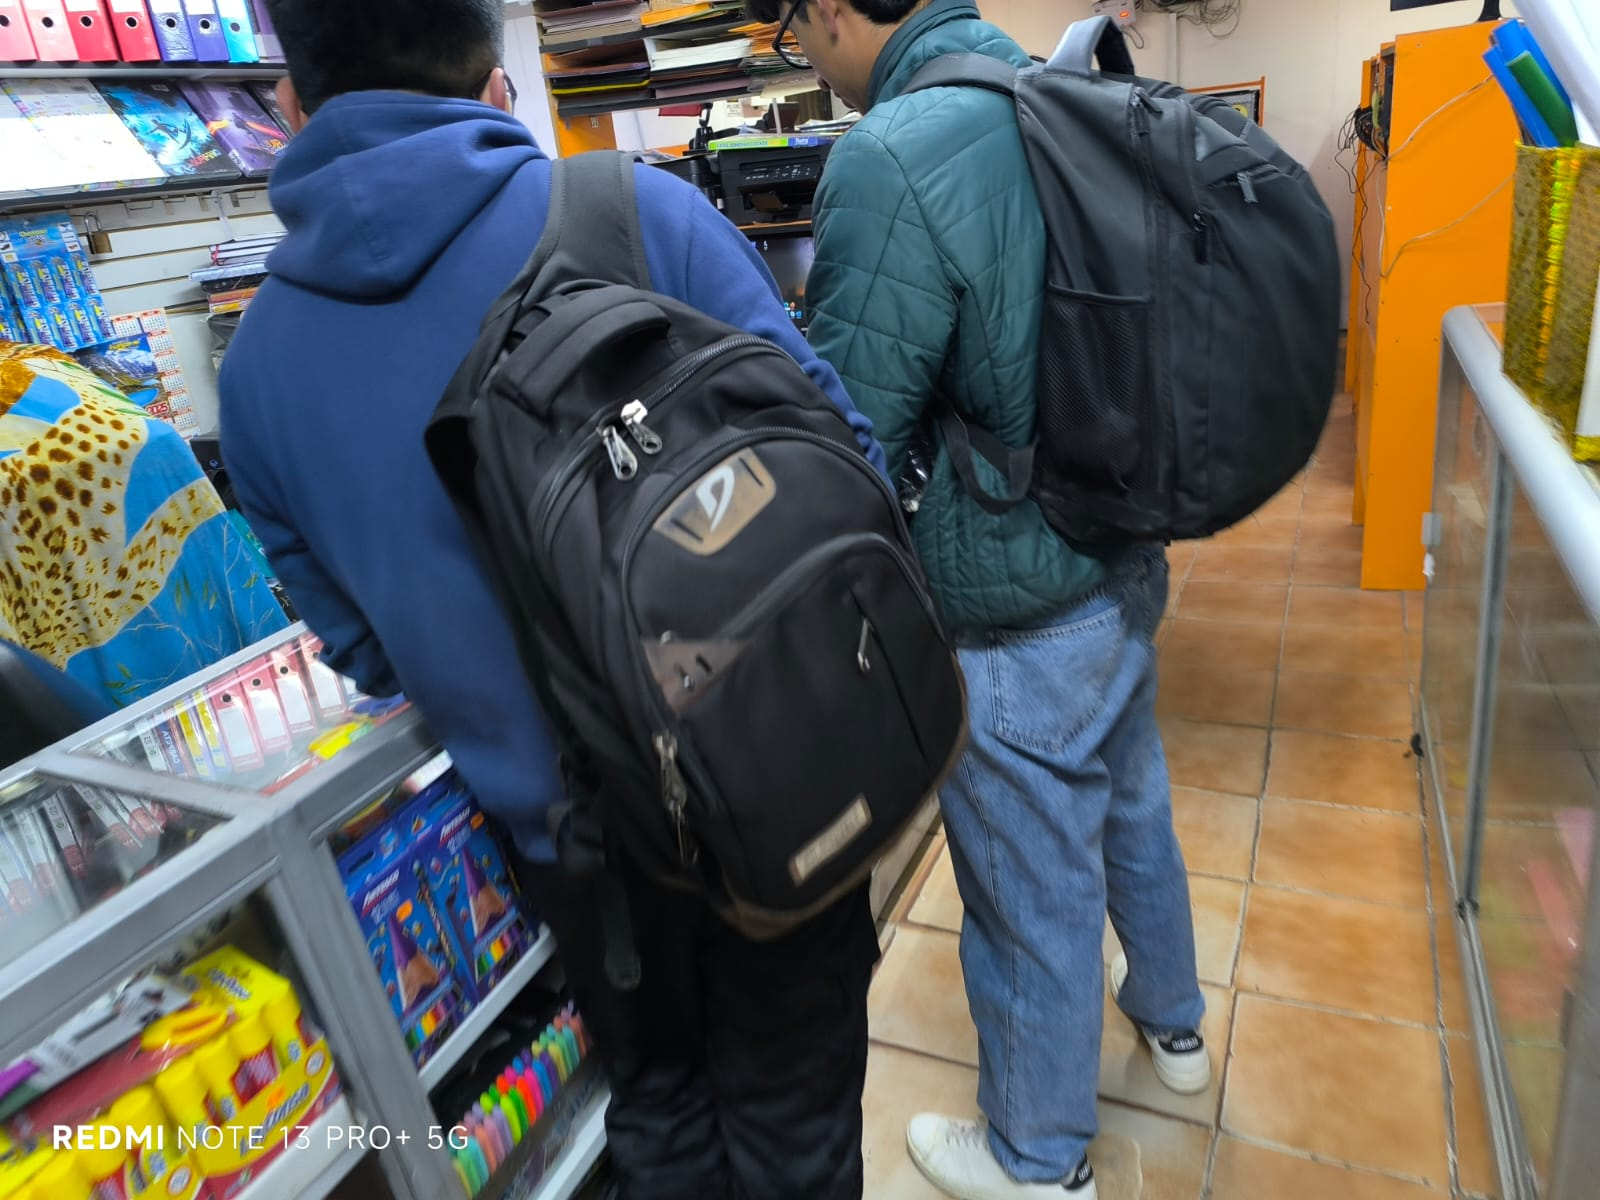
\includegraphics[width=\textwidth]{1.jpeg}
  
\end{minipage}
\hfill
\begin{minipage}[b]{0.48\textwidth}
  \centering
  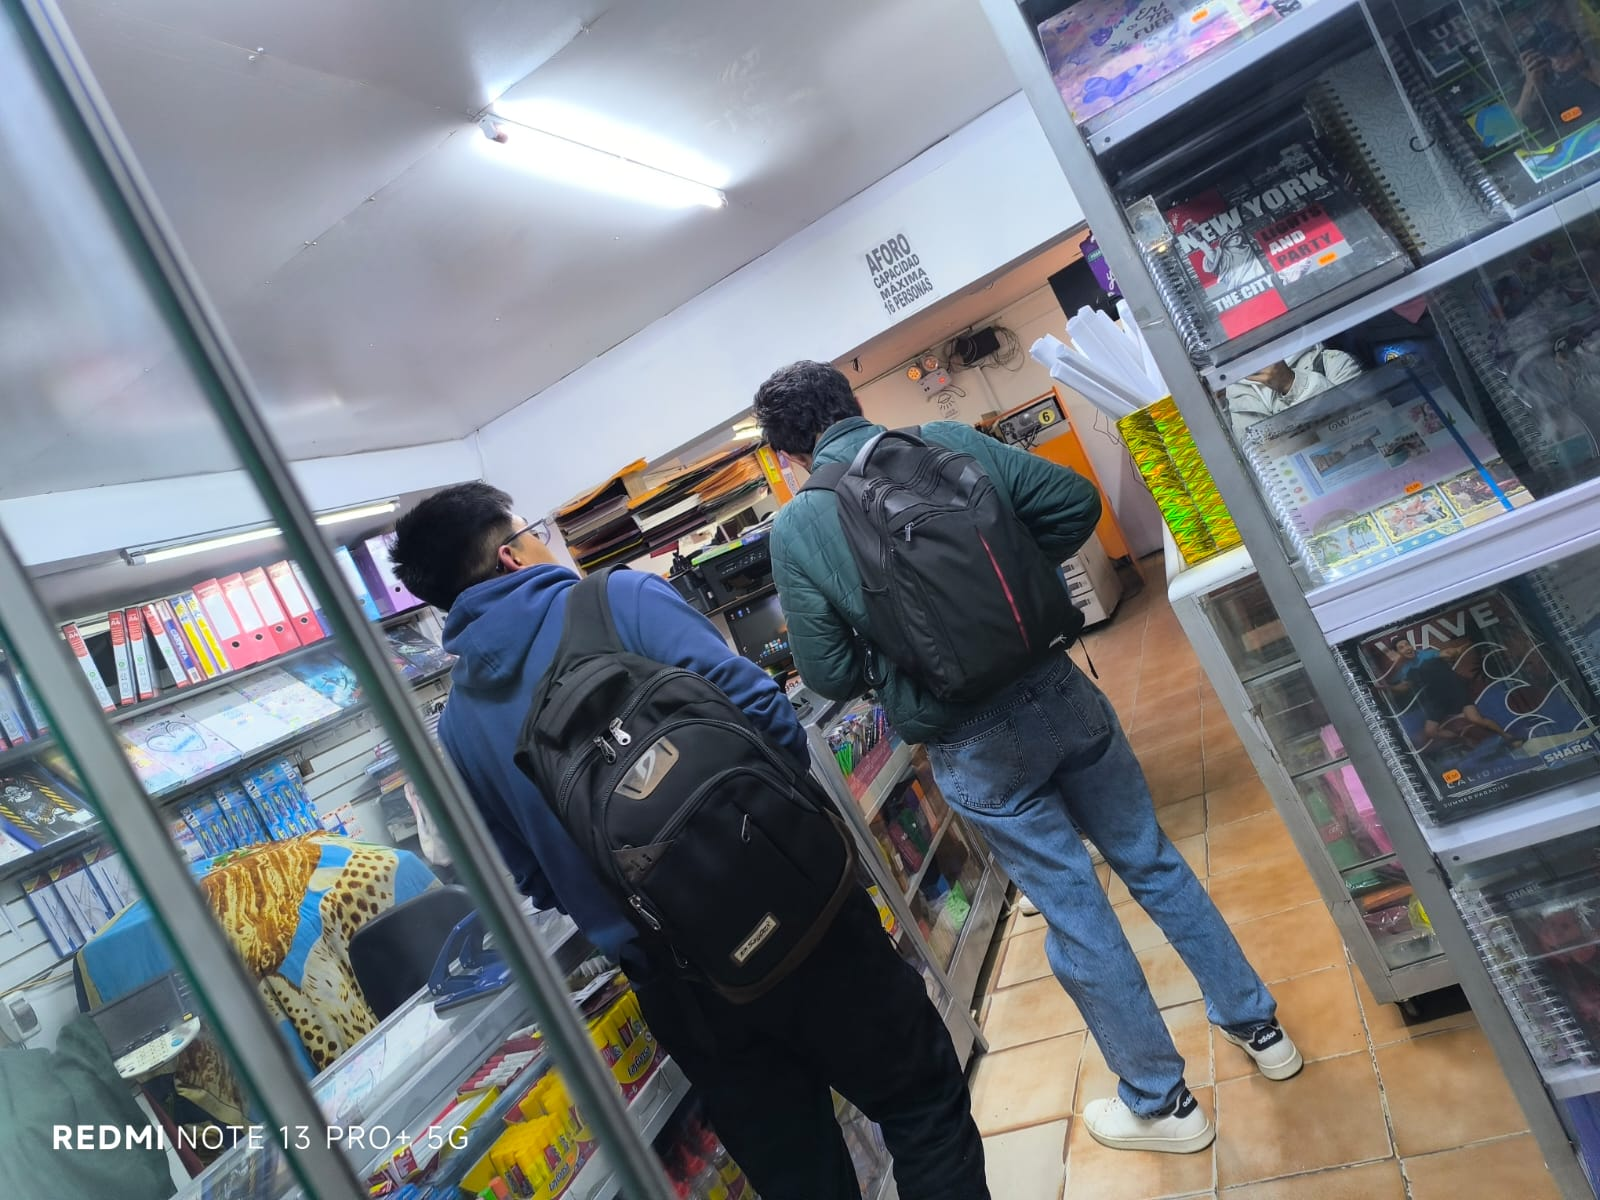
\includegraphics[width=\textwidth]{2.jpeg}
 
\end{minipage}

\vspace{1cm}

% Fila inferior
\begin{minipage}[b]{0.48\textwidth}
  \centering
  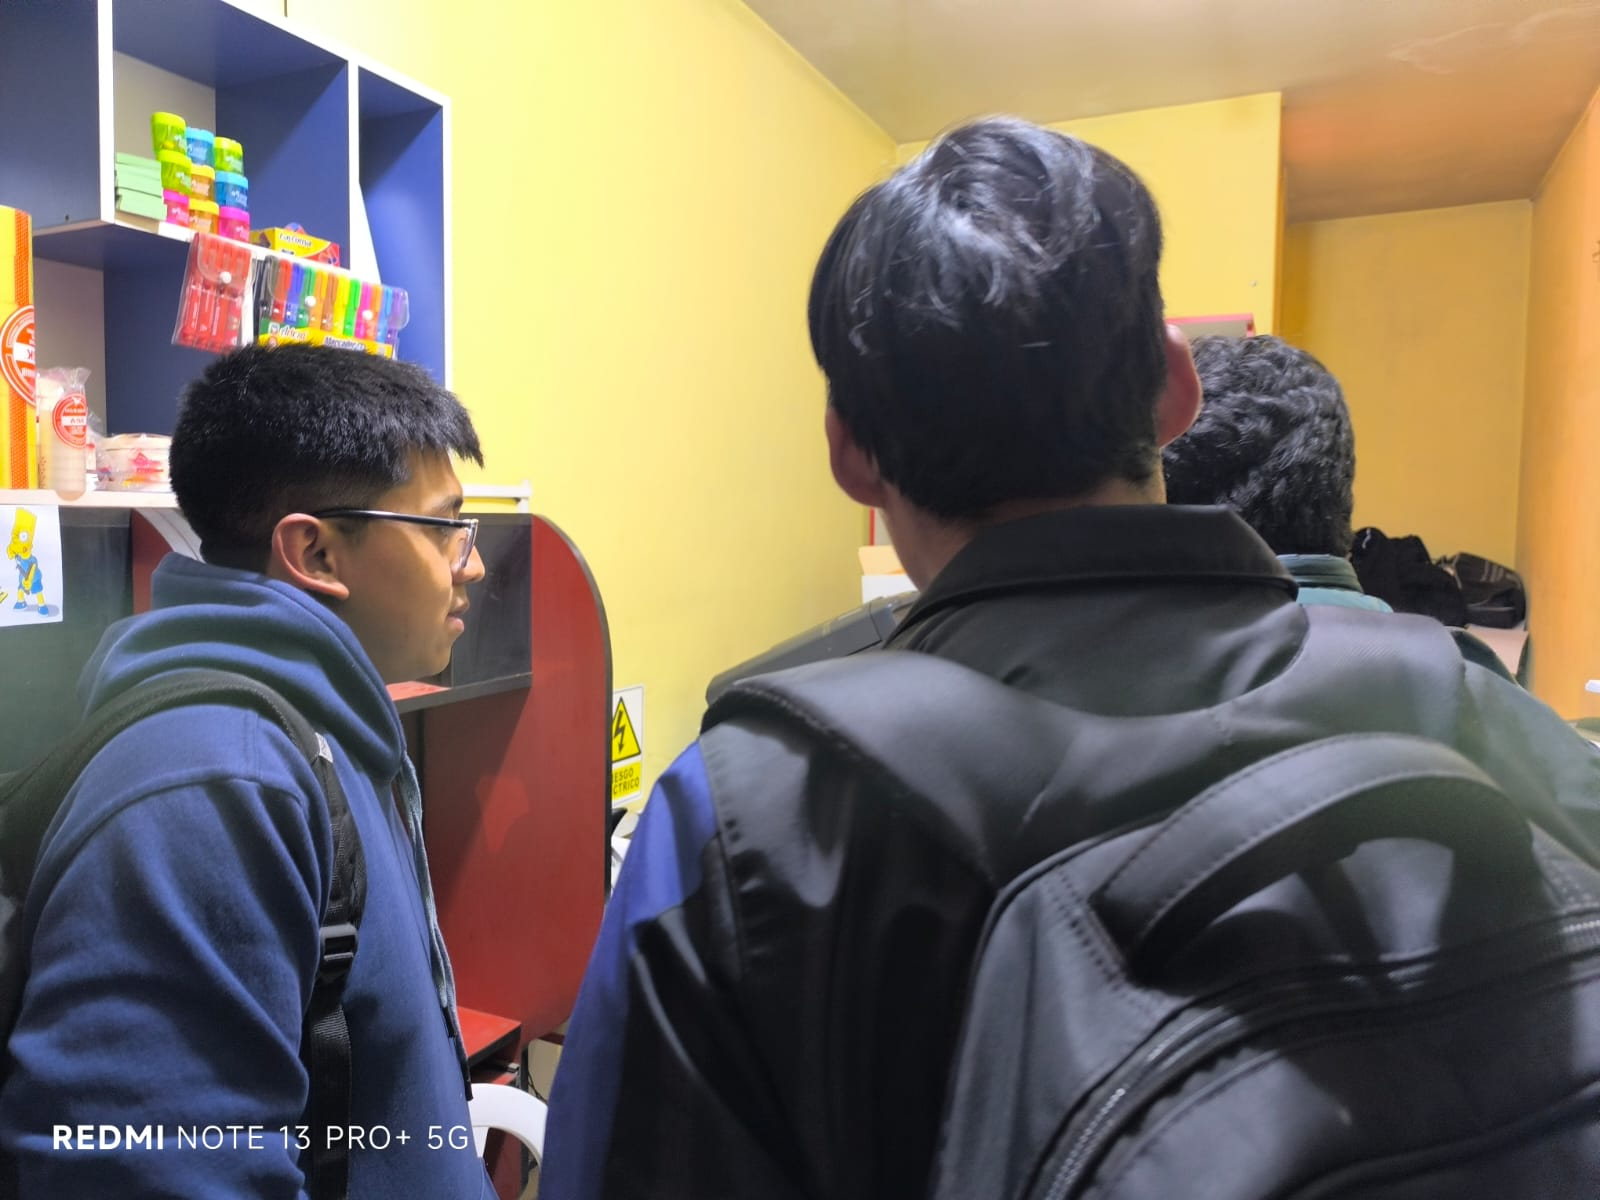
\includegraphics[width=\textwidth]{3.jpeg}
  
\end{minipage}
\hfill
\begin{minipage}[b]{0.48\textwidth}
  \centering
  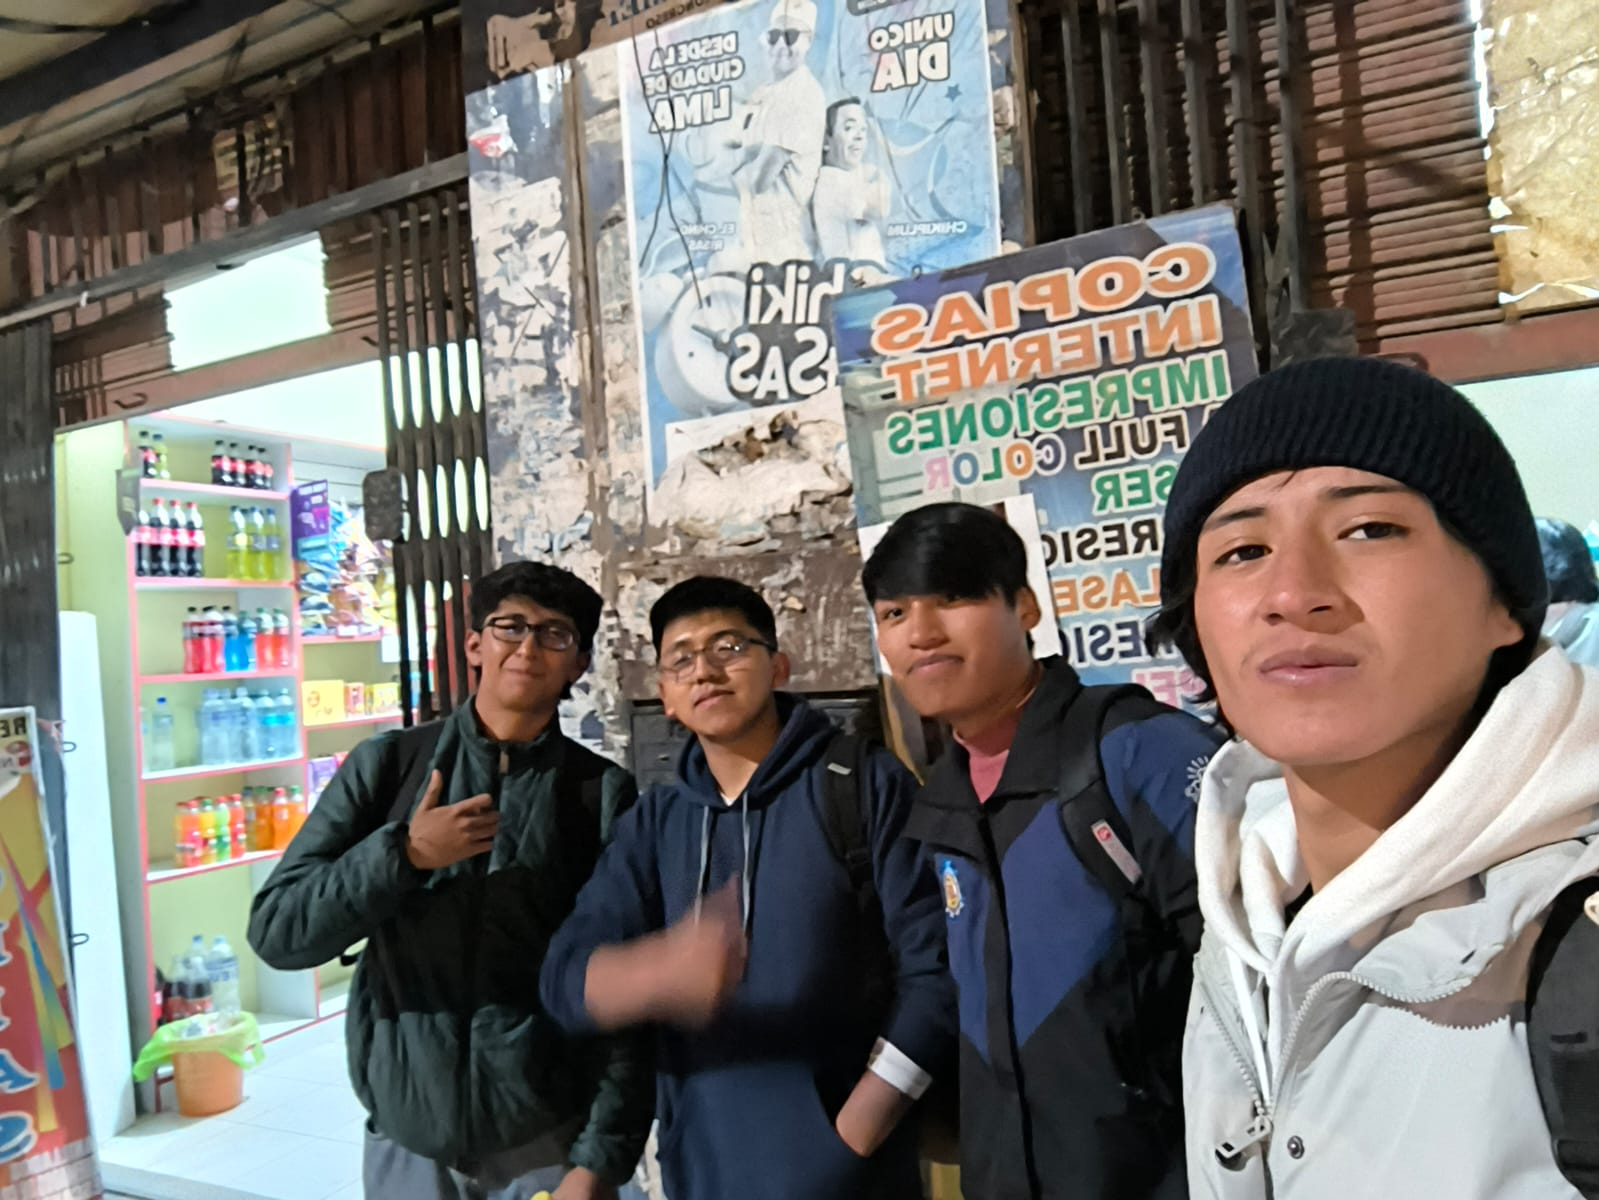
\includegraphics[width=\textwidth]{4.jpeg}
 
\end{minipage}

\end{figure}

\newpage % Para la siguiente página con otras 4 imágenes
\begin{figure}[htbp]
\centering
\begin{minipage}[b]{0.48\textwidth}
  \centering
  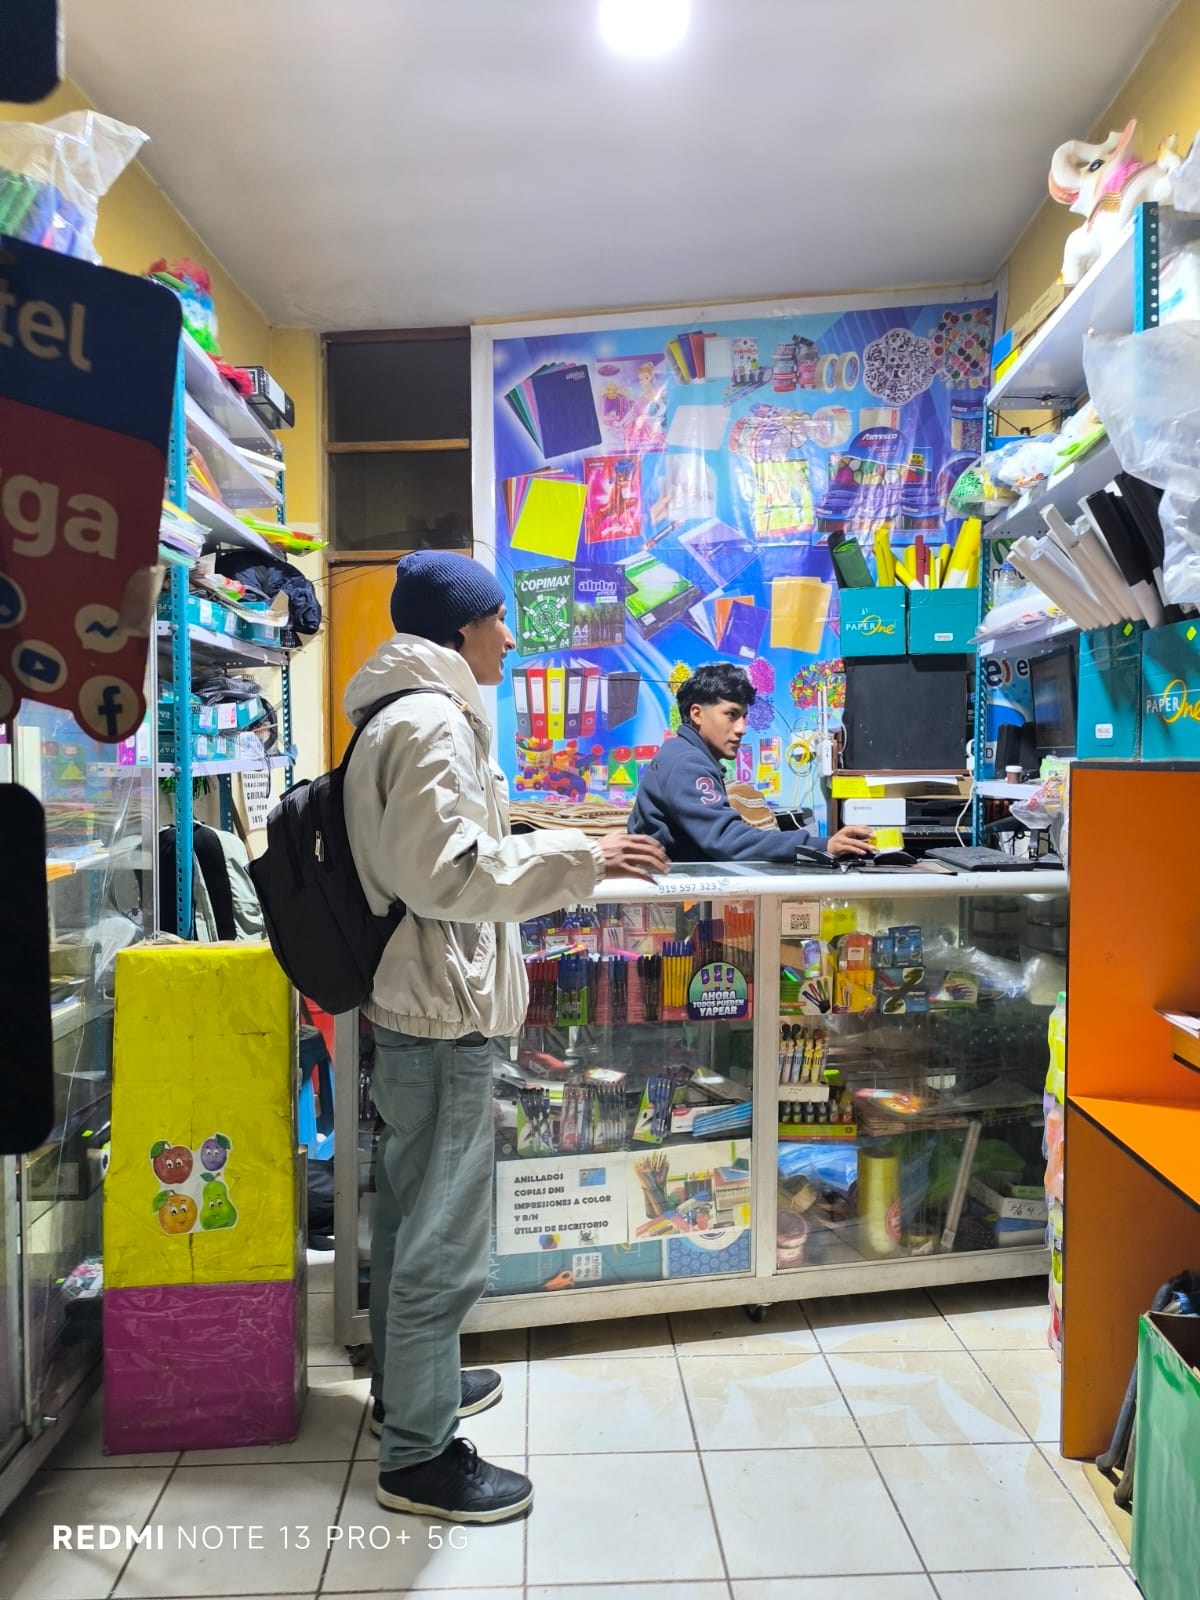
\includegraphics[width=\textwidth]{5.jpeg}
 
\end{minipage}
\hfill
\begin{minipage}[b]{0.48\textwidth}
  \centering
  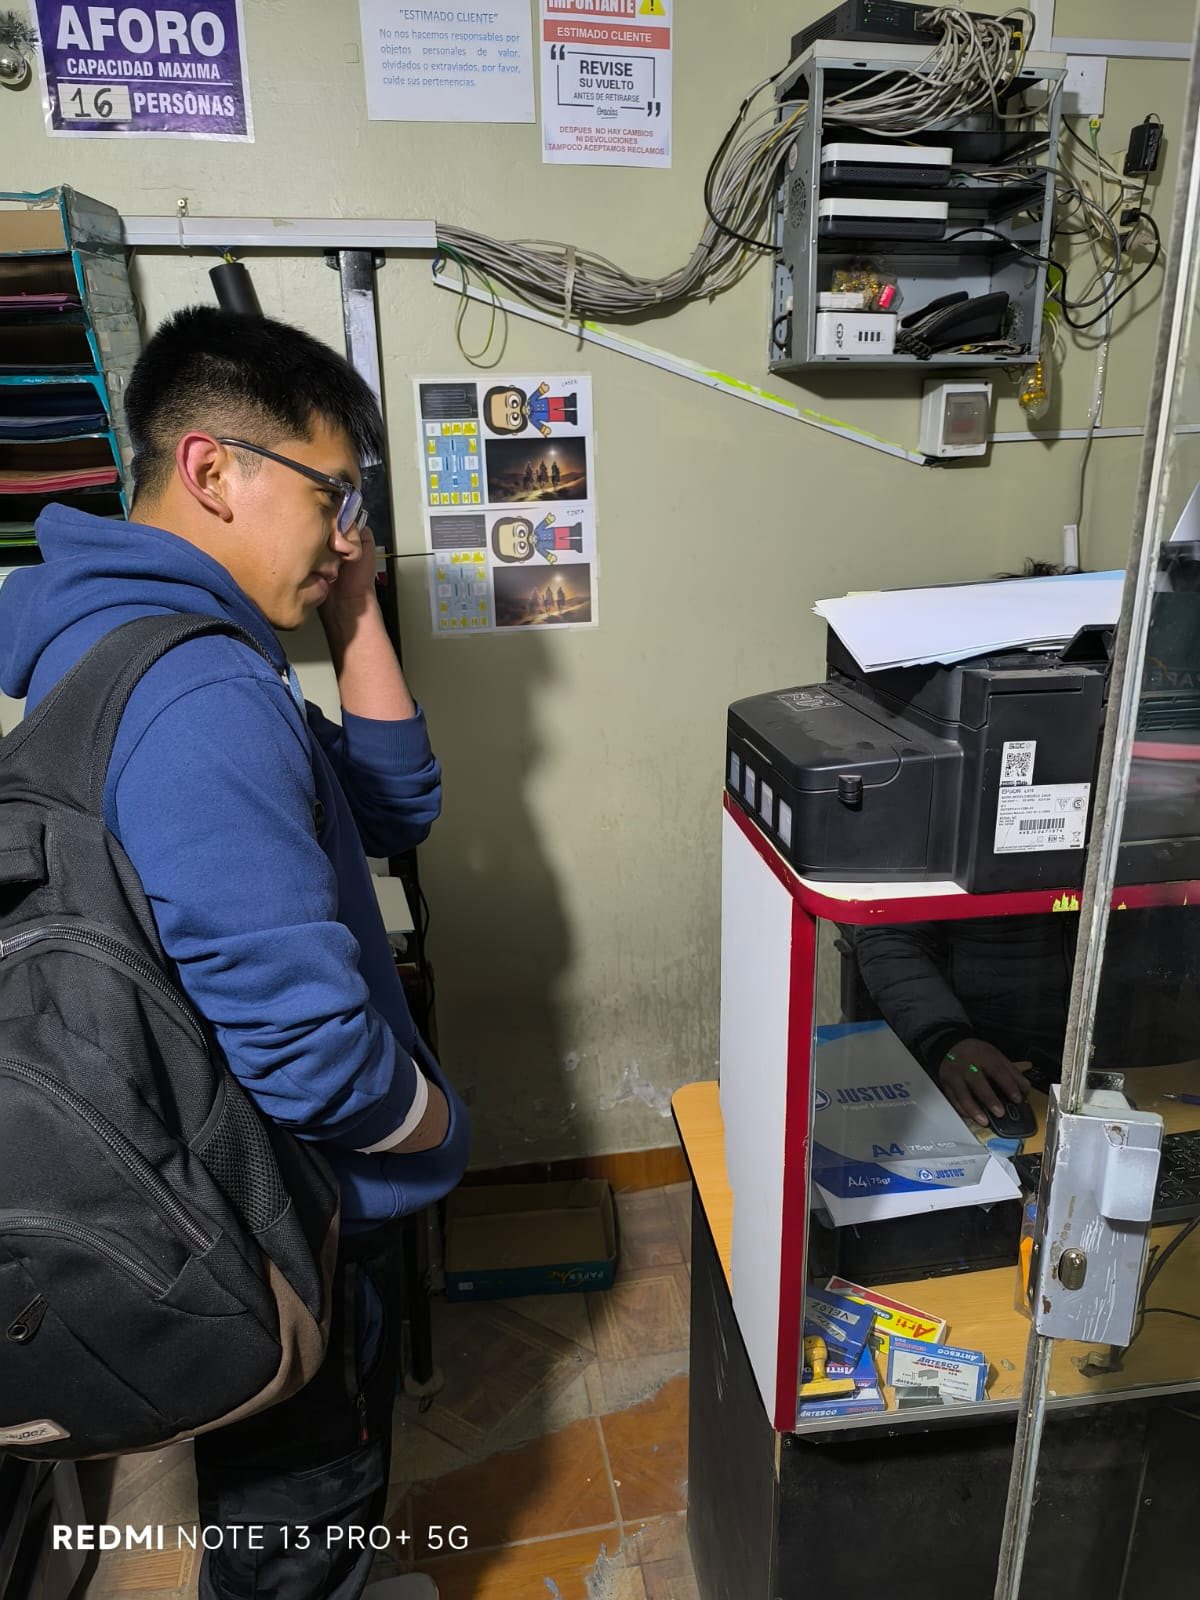
\includegraphics[width=\textwidth]{7.jpeg}
  
\end{minipage}

\vspace{1cm}
\end{figure}
\end{document}